% IEEE-formatted LaTeX paper for Cold Email Generator project
\documentclass[conference]{IEEEtran}
\IEEEoverridecommandlockouts

% Packages
\usepackage[utf8]{inputenc}
\usepackage[T1]{fontenc}
\usepackage{graphicx}
\usepackage{amsmath}
\usepackage{hyperref}
\usepackage{listings}
\usepackage{cite}
\usepackage{xcolor}

\hypersetup{
  colorlinks=true,
  linkcolor=blue,
  citecolor=blue,
  urlcolor=blue
}

% Title and Author
\title{Cold Email Generation with Hybrid LLM Providers and Chroma-based Retrieval}

\author{\IEEEauthorblockN{Soham Pal}
\IEEEauthorblockA{\textit{Independent Researcher} \\
Email: soham@example.com}
}

\begin{document}
\maketitle

\begin{abstract}
This paper presents a practical system for generating professional cold emails tailored to job descriptions. The system combines retrieval from a portfolio vector store backed by ChromaDB with large language models (LLMs), supporting multiple providers (OpenAI and Google Gemini) with robust fallback. We describe the architecture, implementation details, and empirical results from smoke tests, along with engineering lessons on dependency management, reproducibility, and telemetry suppression.
\end{abstract}

\begin{IEEEkeywords}
Cold email generation, Large language models, Retrieval-Augmented Generation, ChromaDB, LangChain, Flask
\end{IEEEkeywords}

\section{Introduction}
Cold outreach remains a crucial business development practice. However, crafting concise, personalized emails is time-consuming. Recent advances in LLMs enable high-quality text generation, but reliability, cost, and provider constraints (e.g., quotas) can hinder adoption. We present an end-to-end system that:
\begin{itemize}
  \item Parses job descriptions and extracts key attributes (role, experience, skills, description).
  \item Retrieves relevant portfolio links using a ChromaDB vector store.
  \item Generates a professional email using an LLM, with a provider-fallback mechanism.
\end{itemize}
The system is implemented with LangChain~\cite{langchain}, Flask~\cite{flask}, and ChromaDB~\cite{chromadb}, supporting both OpenAI~\cite{openai} and Google Generative AI (Gemini)~\cite{gemini}.

\section{Related Work}
Retrieval-Augmented Generation (RAG) is widely used to ground LLM outputs in enterprise context. Our design aligns with practical RAG systems that index domain artifacts and condition LLMs with retrieved evidence. Provider-agnostic interfaces, as popularized by toolkits (e.g., LangChain), reduce vendor lock-in and improve resilience.

\section{System Architecture}
Figure~\ref{fig:arch} illustrates the architecture. A CSV portfolio is ingested into ChromaDB as a persistent collection. The web application accepts a JSON payload describing a job, retrieves relevant links, and invokes an LLM chain to produce the email. The LLM is selected via environment variables with a robust fallback between OpenAI and Gemini.

\begin{figure}[t]
  \centering
  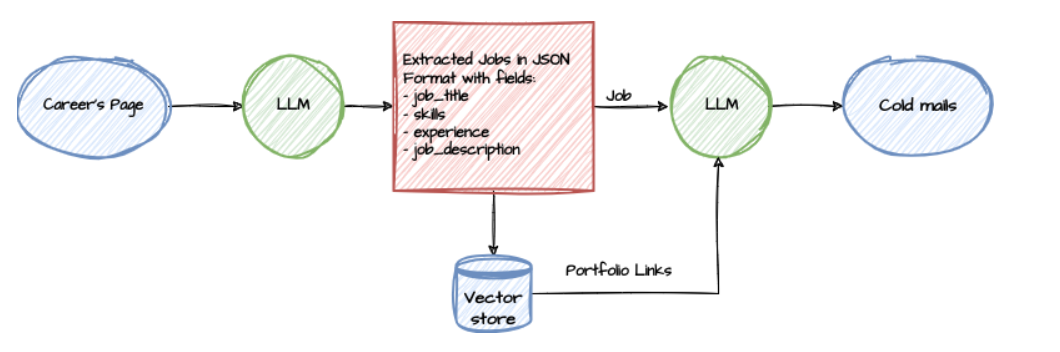
\includegraphics[width=0.48\textwidth]{../imgs/architecture.png}
  \caption{High-level system architecture.}
  \label{fig:arch}
\end{figure}

\section{Methodology}
\subsection{Data Ingestion}
We parse the portfolio CSV (tech stack and links) and populate a Chroma collection (\texttt{portfolio}). We disable anonymized telemetry and validate persistence with a guarded \texttt{count()} call; on failure, we fall back to a fresh path.

\subsection{Vector Retrieval}
Given job skills, we build a query string and issue a nearest-neighbor query over the \texttt{portfolio} collection to obtain \textit{n} link metadata entries.

\subsection{LLM Provider Abstraction}
We expose a function \texttt{initialize\_llm()} that loads provider and model information from environment variables. The system prefers the configured provider (OpenAI or Gemini) and falls back to the other if initialization fails (e.g., quota or missing key). We use LangChain integrations for both providers.

\subsection{Email Generation Chain}
We template the prompt with role, experience, skills, description, and formatted portfolio links. The chain is executed through the chosen \texttt{Chat} interface, returning compact, professional emails under 200 words with a clear CTA.

\section{Implementation}
\subsection{Repository Structure}
Key components:\\
\texttt{emailgen.py}: CLI generation with provider fallback and robust Chroma init.\\
\texttt{webapp/app.py}: Flask web server exposing \texttt{/generate-email}.\\
\texttt{app/chains.py, app/utils.py}: Helper chains and utilities.\\
\texttt{vectorstore/}: Persistent Chroma store.

\subsection{Dependency Management}
We pin key library versions to avoid incompatibilities. Shared dependencies are centralized in \texttt{requirements-common.txt} and included from root and webapp requirements to prevent drift. We discovered specific constraints: aligning \texttt{langchain-*} adapters with \texttt{openai} 1.x and pinning Werkzeug 2.2.x for Flask 2.0.x testing.

\subsection{Telemetry and Logging}
To reduce noisy logs, we disable anonymized Chroma telemetry, set environment variables (\texttt{CHROMA\_TELEMETRY\_DISABLED=true}, \texttt{POSTHOG\_DISABLED=true}), and set logger levels for \texttt{chromadb} and \texttt{opentelemetry} to ERROR.

\section{Experiments and Results}
We performed smoke tests using a Gemini API key due to OpenAI quota constraints. The web app returned successful 200 responses for both the index route and the email generation endpoint, producing coherent emails grounded with retrieved links. While some third-party warnings persisted (e.g., gRPC ALTS messages), they did not affect functionality.

\subsection{Qualitative Output}
Emails were concise (\textless{}200 words), tailored to role and skills, and included portfolio links. The tone was professional with clear CTAs.

\section{Discussion}
\subsection{Limitations}
- No quantitative evaluation beyond smoke testing.
- Portfolio retrieval quality depends on CSV content and embedding configuration (default settings).
- Residual third-party warnings persist despite suppression.

\subsection{Future Work}
- Add evaluation metrics (readability, relevance) and A/B testing.
- Tune embeddings and similarity metrics; add chunking and richer metadata.
- Expand UI for link preview and subject line variants; add provider selection per request.

\section{Conclusion}
We delivered a reliable cold email generation system with provider fallback and robust Chroma integration. The design emphasizes resilience, reproducibility, and practical engineering, offering a template for similar LLM-backed applications.

\section*{Acknowledgments}
We thank the open-source communities behind LangChain, ChromaDB, and Flask.

\bibliographystyle{IEEEtran}
\bibliography{references}

\end{document}
